\section{Learning Phase}
In this section, we describe the learning phase of our technique where we collect the triplets (initial rating, final rating, and observed median) for building our model.
We will explain in detail the system design of the California Report Card, how we record changed ratings, and define the notation that we will use in the following sections.

\subsection{The California Report Card}
The California Report Card (CRC) \footnote{This study was approved by our Human Subjects committee as per IRB Protocol 2014-01-5918.} is a prototype cross-platform web/mobile application designed to allow participants to advise California state leaders on timely policy issues.
The CRC extends our earlier work with Opinion Space and Eigentaste \cite{faridani2011using, bitton2009spatial, faridani2010opinion, nathanson2007eigentaste, goldberg2001eigentaste}.
In the CRC, participants assign letter grades (A+ to F) to the state of California on the following six issues: (1) Implementation of the Affordable Care Act (``Obamacare"),
(2) Quality of K-12 public education, (3) Affordability of state colleges and universities, (4) Access to state services for undocumented immigrants, (5) Laws and regulations regarding recreational marijuana, and (6) Marriage rights for same-sex partners.
Grades (Ratings) are assigned on a thirteen point scale (A+,A,A-,...,D-,F).
These issues are posed in a fixed order each with the same input scale.
Participants submit ratings using a click-and-drag slider interface as illustrated in Figure \ref{grading-1}.
On mobile devices, participants touch and drag to indicate the desired rating.

\begin{figure}[h]
  \centering
    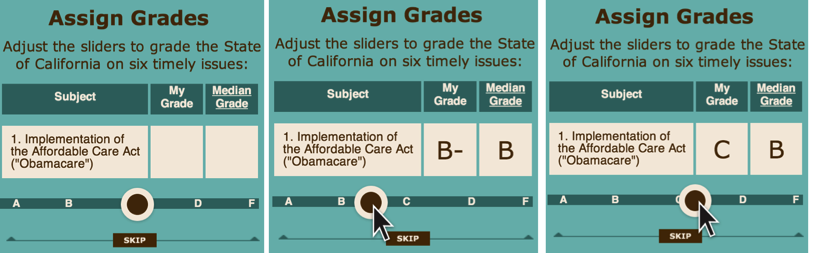
\includegraphics[scale=0.40]{../plots/grading-desc-1.png}
      \caption{After entering their rating, the median rating over all participants is revealed. Participants have the option to change their rating after seeing the median.}
      \label{grading-1}
\end{figure}

Upon release of the slider, the CRC reveals the median for that issue over all prior participants.
Even after the median is revealed the slider is still active and participants can change their ratings.
However, it is important to note that participants were not explicitly told that they could change their rating.
Another important observation is that participants who accessed the application at different times may have seen different medians as they were calculated based on the data up to that point.
We recorded the initial rating, the median that the participant observed, and any subsequent changes along with timestamps for each of the events. 
Rating all of the six issues was not mandatory and participant had the option to skip any of the issues.
To analyze this data, we mapped these 13 grade values linearly onto a scale from 0 to 1, with 1 being an A+ and 0 being an F.

\subsection{Notation}
Let $P$ denote the set of all participants.
For each participant $p_j\in P$, we associate a 3-tuple of ratings ($g_i[j]$, $m[j]$, $g_f[j]$) which represent the initial rating, median observed by the participant, and the final rating.
For each issue, we divided the participants into three subsets of $P$: ones who did not change their ratings $P_n$, ones who changed $P_c$, and ones who skipped the question $P_s$.
Our primary objective is to test the distributional properties of rating tuples from participants in $P_n$ compared to those in $P_c$.

To ensure that all participants in the set $P_c$ had an opportunity to see the median and then react, we filtered this group using the timestamps. 
The median appears in the interface with an animation whose completion time varied between devices, so we set a grace period of 3 seconds before 
we categorized the participant into set $P_c$.  

For consistency, we use the same notation to describe participants in the reference survey. We denote the set of reference survey participants as set $R$, and each participant is associated with a 3-tuple ($g_i[j]$, $m[j]$, $g_f[j]$). However, since the reference survey does not reveal the median $g_i[j] = g_f[j]$  and $m[j]$ is the hypothetical median of the prior participants (which is not shown).
